\section{Topologies} 

  \subsection{Open Sets} 

    \begin{definition}[Topology]
      Let $X$ be a set and $\mathscr{T}$ be a family of subsets of $X$. Then $\mathscr{T}$ is a \textbf{topology} on $X$\footnote{I will use script letters to denote topologies and capital letters to denote sets.} if it satisfies the following properties. 
      \begin{enumerate}
        \item \textit{Contains Empty and Whole Set}: 
        \begin{equation}
          \emptyset, X \in \mathscr{T}
        \end{equation}

        \item \textit{Closure Under Union}. If $\{U_\alpha\}_{\alpha \in A}$ is a class of sets in $\mathscr{T}$, then 
        \begin{equation}
          \bigcup_{\alpha \in A} U_\alpha \in \mathscr{T}
        \end{equation}

        \item \textit{Closure Under Finite Intersection}: If $U_1, \ldots, U_n$ is a finite class of sets in $\mathscr{T}$, then 
        \begin{equation}
         \bigcap_{i=1}^{n} U_i \in \mathscr{T}
        \end{equation}
      \end{enumerate}
      A \textbf{topological space} is denoted $(X, \mathscr{T})$. 
    \end{definition}

    This leads to the most general definition of an open set. 

    \begin{definition}[Open Set]
      The elements of $\mathscr{T}$ are called \textbf{open sets} in $X$.\footnote{As implied from the definition of a topology, the arbitrary union and finite intersection of any number of open sets is an open set.} 
      \begin{enumerate}
        \item An open set $U$ which contains a point $x$ is called an \textbf{open neighborhood} of $x$, denoted $U_x$. 
        \item Given an open neighborhood $U_x$ of $x$, the set $U_x \setminus \{x\}$ is called the \textbf{punctured open neighborhood} of $x$. 
      \end{enumerate}
    \end{definition}

    Note that an open set doesn't really mean anything without talking about with respect to its topology. 

    Note that we restrict property 3 to be a \textbf{finite} intersection because if we don't, the open ball topology on $\mathbb{R}$ would imply that 
    \begin{equation}
      \bigcap_{i = 1}^{\infty} \Big( - \frac{1}{i}, \frac{1}{i} \Big) = 0
    \end{equation}
    is an open set $\implies$ all points are open sets too, which can be troublesome for later purposes. 

    \begin{example}[Topologies of a Set of Cardinality 3]
      There are a total of 29 topologies that we can construct on $\{1, 2, 3\}$. Two such examples are 
      \begin{enumerate}
        \item $\{\emptyset, \{1, 2\}, \{1, 2, 3\}\}$ 
        \item $\{\emptyset, \{3\}, \{2, 3\}, \{1, 2, 3\}\}$
      \end{enumerate}
    \end{example} 

    \begin{theorem}[Discrete, Indiscrete Topologies]
      Given a set $X$, 
      \begin{enumerate}
        \item $2^X$ is a topology, called the \textbf{discrete topology}. 
        \item $\{\emptyset, X \}$ is a topology, called the \textbf{indiscrete topology}. 
      \end{enumerate}
    \end{theorem}
    \begin{proof}
      Listed. 
      \begin{enumerate}
        \item The first property is trivially proven. From the theorems of set theory, $U_\alpha \subset X \implies \cup U_\alpha \subset X \implies \cup U_\alpha \in 2^X$. Finally the same logic holds for intersection as well. 
        \item The first property is trivially proven. We can check for the 4 combinations of unions and intersections and see that they all result in either $\emptyset$ or $X$. 
      \end{enumerate}
    \end{proof}

    Note that we don't need to have any structure (e.g. order, metric, measure) on our set $X$ to define a topology. Two trivial examples were shown above, but there are some interesting ones. 

    \begin{theorem}[Cofinite Topology]
      Given a set $X$, the set of all subsets $U$, satisfying the property that $X \setminus U$ is finite, is a topology, called the \textbf{cofinite topology} or the \textbf{finite complement topology}.\footnote{While this definition may seem a bit arbitrary, this is very similar to the Zariski topology, which is used in algebraic topology.} 
    \end{theorem}
    \begin{proof}
      Let us denote this set $\mathscr{T}_c$. 
      \begin{enumerate}
        \item By definition $\emptyset \in \mathscr{T}_c$. It is clear that $X \setminus X = \emptyset$ has cardinality $0$, and therefore is in $\mathscr{T}_c$. 

        \item Let $\{U_\alpha\}_{\alpha \in I} \in \mathcal{T}_c$ by a collection of open sets of $X$. Then by deMorgan's laws, 
        \begin{equation}
          X \setminus \bigcup_{\alpha \in I} U_{\alpha} = \bigcap_{\alpha \in I} (X \setminus U_\alpha)
        \end{equation}
        $X \setminus U_\alpha$ is countable for all $\alpha \in I$, so let us fix some $\alpha^\prime$. Then 
        \begin{equation}
          \bigcap_{\alpha \in I} (X \setminus U_\alpha) \subset U_{\alpha^\prime} \implies \bigg| \bigcap_{\alpha \in I} (X \setminus U_\alpha) \bigg| \leq \big| U_{\alpha^\prime} \big| 
        \end{equation}
        and so the intersection is also countable. 

        \item Let $\{U_i\}_{i=1}^n$ by a finite collection of open sets of $X$. Then by deMorgan's laws, 
        \begin{equation}
          X \setminus \bigcap_{i=1}^n U_i = \bigcup_{i=1}^n (X \setminus U_i)
        \end{equation}
        Since $U_i$ are open, $X \setminus U_i$ are countable, and since the finite union of countable sets are countable, the RHS is countable, which implies the LHS is countable and so $\cap_{i=1}^n U_i$ is open as well. 
      \end{enumerate}
    \end{proof} 

    Slightly modifying the definition does not result in a topology. 

    \begin{example}[Countable Complement is Not A Topology]
      Given a set $X$, consider the collection 
      \begin{equation}
        \mathscr{T}_\infty \coloneqq \{U \subset X \mid X \setminus U \text{ is infinite or empty or all of }X \}
      \end{equation}
      This is not a topology. Let us take $X = \mathbb{R}$, and look at the sets $\mathbb{Z}_{\geq 0}, \mathbb{Z}_{\leq 0}$ consisting of all the non-negative and non-positive integers. They are both infinite, and so $\mathbb{R} \setminus \mathbb{Z}_{\geq 0}$ and $\mathbb{R} \setminus \mathbb{Z}_{\leq 0}$ are in $\mathcal{T}_\infty$. Consider their union. 
      \begin{equation}
        (\mathbb{R} \setminus \mathbb{Z}_{\geq 0}) \cup (\mathbb{R} \setminus \mathbb{Z}_{\leq 0}) = \mathbb{R} \setminus (\mathbb{Z}_{\geq 0} \cap \mathbb{Z}_{\leq 0}) = \mathbb{R} \setminus \{0\}
      \end{equation}
      But $\mathbb{R} \setminus (\mathbb{R} \setminus \{0\}) = \{0\}$, and so $\mathbb{R} \setminus \{0\}$ is not open. Therefore $\mathcal{T}_c$ doesn't satisfy the definition of a topology. 
    \end{example}

    For common sets like $\mathbb{R}^n$, which has an inner product, or $\mathbb{Q}$, which has an order, it is easy to build these topologies with set-builder notation. Consider the following. 

    \begin{theorem}[Metric Topology]
      Given a metric space $(X, d)$, let us denote the \textbf{metric topology}, or \textbf{open-ball topology}, as the set of subsets $U$ satisfying the property that for all $x \in U$, there exists a positive $r \in \mathbb{R}$ such that $B(x, r) \subset U$, where $B(x, r) \coloneqq \{y \in X \mid d(x, y) < r\}$ is the open ball of radius $r$ around $x$. We claim that this is a topology. 
    \end{theorem} 
    \begin{proof}
      We show that the properties of a topology hold. 
      \begin{enumerate} 
        \item For the empty set, the inclusion of an open ball for a point in $\emptyset$ is vacuously satisfied. For the whole set, we choose any point $x$ and any $r$, and the open ball is trivially a subset of $X$. 

        \item Let $\{U_\alpha\}_{\alpha \in I}$ be a collection of open subsets of $X$. Let their union be denoted $U$. We claim $U$ is open. Pick any point $x \in U$. Then by definition of union, there exists some $\alpha \in I$ s.t. $x \in U_\alpha$. Since $U_\alpha$ is open, there exists a $r > 0$ s.t. $B(x, r) \subset U_\alpha \subset U$. Therefore $U$ is open. 

        \item Let $U_1, \ldots, U_k$ be open, and let us denote their intersection as $U$. We claim $U$ is open. Pick a point $x \in U$. Then for each $i = 1, \ldots, k$, $x \in U_i$ and there exists a corresponding $r_i > 0$  such that the open ball $B(x, r_i) \subset U_i$. Take the set $R = \{r_i\}$, which is a finite set living in $\mathbb{R}$. We will take for granted that every finite subset of an ordered set has a minimum.\footnote{If we wish to prove it, we can start with a singleton set, claim that its minimum is the only element. Then we use induction by assuming for a set $R$ of size $k$ that a minimum exists, and by adding $1$ more element $r$ we update the minimum to be $\min\{r, \min{R}\}$ and show that this is indeed the minimum.} Let us denote $r^\ast = \min{R}$, and we claim that $r^\ast$ gives us a ball that can fit inside $U$. Assume $y \in B(x, r^\ast)$. Then 
        \begin{align}
          y \in B(x, r^\ast) & \implies d(x, y) < r^\ast \\ 
                             & \implies d(x, y) < \min{R} \\
                             & \implies d(x, y) < r_i \text{ for } i = 1, \ldots, k \\
                             & \implies y \in B(x, r_i) \text{ for } i = 1, \ldots, k
        \end{align} 
        Since $B(x, r_i)$ by construction is contained within $U_i$, $y \in U_i$ for all $i$. This means by definition of intersection that $y \in U$, and we have proven that $B(x, r^\ast)$ completely fits inside $U$. 
      \end{enumerate}
    \end{proof} 

    Note that while open balls are used to define whether a set is open or not, the definition doesn't state whether open balls themselves are open sets. It turns out that it is easy to prove that they are. 
    
    \begin{corollary}[Open Balls are Open Sets]
      The open ball w.r.t. to any metric $d$ is an open set w.r.t. to the metric topology. 
    \end{corollary}
    \begin{proof}
      Let $y \in B(x, r)$. Then $d(x, y) < r \implies 0 < r - d(x, y)$. To show that $B(x, r)$ is open, we would like to show that there exists some $r^\prime > 0$ s.t. $y \in B(y, r^\prime) \subset B(x, r)$. Set $r^\prime = r - d(x, y)$. Then 
      \begin{align}
        z \in B(y, r^\prime) & \implies d(y, z) < r - d(x, y) \\
                             & \implies d(x, y) + d(x, y) < r \\
                             & \implies d(x, z) < r \\
                             & \implies z \in B(x, r)
      \end{align} 
      and so $B(y, r^\prime) \subset B(x, r)$. We are done. 
    \end{proof}

    More specifically, the metric topology generated by the $L_2$-metric on $\mathbb{R}^n$ is called the \textbf{Euclidean topology}. Note that the topological property of stability under countable intersection was required to show that the minimum of $R$ existed. This is not true for infinite sets in general. This gives us some motivation as to why we need the \textit{finite} intersection rather than an infinite one. 
    
    \begin{corollary}[Singletons are Not Open in $\mathbb{R}^n$]
      A singleton set is not open in $\mathbb{R}^n$ with the Euclidean topology.   
    \end{corollary}
    \begin{proof}
      We claim that the singleton set $S = \{0\}$ is not open under the Euclidean metric. We pick a point in $S$, which can only be $0$. Assume that there exists an $r > 0$ s.t. $B(x, r) \subset S$. $\mathbb{R}$ is Archimedean, so there exists a natural number $N$ s.t. $0 < 1/N < r$. We construct the vector $v = (v_1, \ldots, v_n)$ s.t. $v_1 = 1/N$ and $v_i = 0$ everywhere else. The distance between $0$ and $v$ is 
      \begin{equation}
        || v - 0 || = ||v|| = \sqrt{(1/N)^2} = 1/N < r
      \end{equation} 
      so $v \in B(x, r)$. But $v \neq 0$, and by contradiction such an $r$ cannot exist. In $\mathbb{R}^n$ we consider the countable intersection of open balls (which we have proved in class are open sets) around $0$ of radius $1/N$ for $n \in \mathbb{N}$. We claim that 
      \begin{equation}
        \bigcap_{n \in \mathbb{N}} B(0, 1/n) = \{0\}
      \end{equation} 
      We see that $1/n$ must always be positive and so $||0 - 0|| = 0 < 1/n$. Therefore the LHS $\supset $ RHS. To see that the intersection contains no other element, consider any vector $v \neq 0$. Then by definition of the metric, $d(v, 0) > 0$. By the Archimedean property, there exists a natural $N \in \mathbb{N}$ s.t. $0 < 1/N < d(v, 0)$, which means that $v \not\in B(0, 1/N)$, and so $v$ cannot be in the intersection. Therefore, the intersection must be $\{0\}$, and we have shown that $B_0$ is not open, so we are done. 
    \end{proof}

    \begin{theorem}[Open Interval Topology]
      In $\mathbb{R}$, let us denote the \textbf{open interval topology} as the set of subsets $U$ satisfying the property that for all $x \in U$, there exists an open interval $(a, b) \coloneqq \{y \in \mathbb{R} \mid a < y < b\}$ containing $x$ that is contained in $U$, i.e. $x \in (a, b) \subset U$. We claim that this is a topology. 
    \end{theorem}
    \begin{proof}
      
    \end{proof}

    Note that if we had used closed balls or intervals, then this wouldn't work because we can pick a point on the ``boundary'' of the open set. We will get to a more rigorous definition of what a boundary is later, but first, we need to learn what it generally means for a point to be infinitesimally close to a set. 

    \begin{definition}[Limit Point]
      Given a topological space $(X, \mathscr{T}$, let $p \in X$ be a point and $S \subset X$ a subset. $p$ is a \textbf{limit point of $S$} if every punctured neighborhood of $p$ intersects $S$.\footnote{Note that limit point are generally used to talk about points that are infinitesimally close to a set $S$. A limit point may not necessarily be in $S$, and a point of $S$ may not necessarily be a limit point. This is why we use a punctured neighborhood, rather than an open neighborhood. For continuity as we will see later, we just talk about neighborhoods since we also claim that the limit exists and the function value is the limit.} 
    \end{definition}

    \begin{example}[Examples of Limit Points]
      What about the limit points that are not in $S$? Generally, there are two instances. 
      \begin{enumerate}
        \item Let $S$ represent the gray area. $B$ is in the ``interior'' of $S$ and therefore is a limit point. $A$ and $C$ are on the ``boundary'' of $S$ yet not in $S$, and we can show that they are limit points as well. 
          
        \begin{figure}[H]
          \centering 
          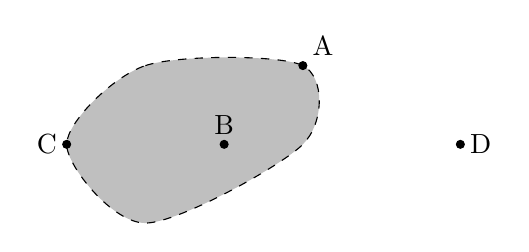
\begin{tikzpicture}
            \draw[fill=lightgray, dashed] plot [smooth cycle] coordinates {(0,0) (1,1) (3,1) (3,0) (1,-1)};
            \draw [fill] (3, 1) circle [radius=0.05];
            \node [above right] at (3,1) {A};
            \draw [fill] (2,0) circle [radius=0.05];
            \node [above] at (2,0) {B};
            \draw [fill] (0,0) circle [radius=0.05];
            \node [left] at (0,0) {C};
            \draw [fill] (5,0) circle [radius=0.05];
            \node [right] at (5, 0) {D};
          \end{tikzpicture}
          \caption{Points $A, B, C$ are limit points of the open set. }
          \label{fig:limit_boundary}
        \end{figure}

        \item A point can be at the ``convergence point'' of a sequence. 
        \begin{figure}[H]
          \centering 
          \begin{tikzpicture}
            \draw [fill] (0, 2.2) circle [radius=0.05];
            \draw [fill] (1, 2.4) circle [radius=0.05];
            \draw [fill] (2, 2) circle [radius=0.05];
            \draw [fill] (2.5, 1.8) circle [radius=0.05];
            \draw [fill] (2.6, 1.6) circle [radius=0.05];
            \draw [fill] (2.65, 1.67) circle [radius=0.05];
            \draw [fill] (2.654, 1.64) circle [radius=0.05];
            \draw [fill] (2.6543, 1.63) circle [radius=0.05];
            \node [right] at (2.6543, 1.63) {p};
          \end{tikzpicture}
          \caption{Note that if $S$ is a sequence of points in $\mathbb{R}^{2}$ that converges to $p$ without ever hitting it, we can say that $p \not\in S$ is a limit point of $S$.}
          \label{fig:limit_sequence}
        \end{figure}
      \end{enumerate}
    \end{example}

    \begin{example}[Examples of Non-Limit Points]
      There are generally two instances of non-limit points. Let $X = \mathbb{R}$ and $S = (0, 1) \cup \{2\}$. 
      \begin{enumerate}
        \item $5$ is clearly not a limit point. 
        \item $2$, although in $S$, is not a limit point since we are talking about the punctured neighborhood. A point in $S$ that is not a limit point is called an \textbf{isolated point}. 
      \end{enumerate}
    \end{example}

  \subsection{Basis} 

    So far so good. We want to continue analyzing the properties of a topology, but sometimes working with the entire topology is a bit thorny. There is a tamer representation of a topology, which can also give us the starting point to \textit{construct} topologies. 

    \begin{definition}[Basis]
      If $X$ is a set, a \textbf{basis} on $X$ is a collection $\mathscr{B}$ of subsets of $X$ (called \textbf{basis elements}) such that
      \begin{enumerate}
        \item For each $x \in X$, there is at least one basis element $B \in \mathscr{B}$ containing $x$. That is, the elements of $\mathscr{B}$ covers $X$. 
        \item If $x$ belongs to the intersection of two basis elements $B_1$ and $B_2$, then there is a basis element $B_3$ containing $x$ such that $B_3 \subset (B_1 \cap B_2)$. 
      \end{enumerate}
    \end{definition} 

    The name gives away the clue that a topology may be created from this basis.  

    \begin{theorem}[Basis to Topology]
      Given a basis $\mathscr{B}$ on a set $X$, we can define a topology $\mathscr{T}$, called the \textbf{topology generated by $\mathscr{B}$}, in the following equivalent ways. 
      \begin{enumerate}
        \item $\mathscr{T}$ consists of subsets $U$ of $X$ satisfying the property that for each $x \in U$, there exists a basis element $B \in \mathscr{B}$ such that $x \in B \subset U$.\footnote{Note that since we can always set $U = \emptyset$, the basis doesn't need to contain $\emptyset$. }
        \begin{center}
          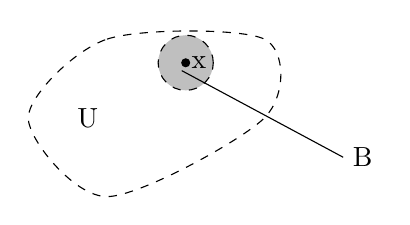
\begin{tikzpicture}
          \draw[dashed] plot [smooth cycle] coordinates {(0,0) (1,1) (3,1) (3,0) (1,-1)};
          \node [right] at (0.5,0) {U};
          \draw[fill=lightgray,dashed] (2,0.7) circle [radius=0.35];
          \draw[fill] (2, 0.7) circle [radius=0.05];
          \node [right] at (1.95,0.7) {x};
          \node [right] at (4,-0.5) {B};
          \draw (1.95,0.6)--(4,-0.5);
          \end{tikzpicture}
        \end{center}

        \item $\mathscr{T}$ consists of all possible unions of elements in $\mathscr{B}$. 
        \begin{equation}
          \mathscr{T} \equiv \Big\{ \bigcup_i b_i \; \Big| \; b_i \in \mathscr{B}\Big\}
        \end{equation}
      \end{enumerate}
    \end{theorem} 
    \begin{proof}
      We prove that the 2 methods generate a topology, and then finally prove that it they are the same topology. 
      \begin{enumerate}
        \item Clearly, $\emptyset$ and $X$ itself are in $\mathscr{T}$. To prove property 2, given a certain indexed family of subsets $\{U_\alpha\}_{\alpha \in I}$ of $\mathscr{T}$, we must show that 
        \begin{equation}
          U = \bigcup_{\alpha \in I} U_\alpha \in \mathscr{T}
        \end{equation}
        Given $x \in U$, there exists at least one index $\alpha$ such that $x \in U_\alpha$. Since $U_\alpha \in \mathscr{T}$ already, there exists a basis element $b \in \mathscr{B}$ such that $x \in b \subset U_\alpha$. But 
        \begin{equation}
          U_\alpha \subseteq U \implies b \subset U
        \end{equation}
        So, by definition, any arbitrary union of $U$ of these subsets is also in $\mathscr{T}$. 

        To prove property 3, we must show that 
        \begin{equation}
          W = \bigcap_{\alpha \in I} U_\alpha \in \mathscr{T}
        \end{equation}
        Given $x \in W$, by definition of a basis element, there exists a $b \in \mathscr{B}$ such that 
        \begin{equation}
          x \in b \subset (U_\beta \cap U_\gamma) \forall \beta, \gamma \in I \implies \text{ there exists } \Tilde{b} \in \mathscr{B} \text{ s.t. } x \in \Tilde{b} \subset \bigcap_{\alpha \in I} U_\alpha
        \end{equation}
        By definition, $W$ is also open. Since this arbitrary set of subsets $\mathscr{T}$ suffices the 3 properties, it is a topology of $X$ by definition. 

        \item $(\rightarrow)$ Given a collection of elements in $\mathscr{B}$, they are also elements of $\mathscr{T}$. Since $\mathscr{T}$ is a topology, their union in also in $\mathscr{T}$. 

        $(\leftarrow)$ Given an open set $U \in \mathscr{T}$, for every point $x \in U$, by definition we can choose a basis element $b \in \mathscr{B}$ such that $x \in b \subset U$. Then, the union of all these basis elements is by definition $b$. 
          
      \end{enumerate}
    \end{proof}

    We have learned how to go from a basis to a topology. The following lemma tells us how to identify a basis within a topology. 

    \begin{theorem}[Topology to Basis]
      Let $X$ be a topological space, and let $\mathcal{C}$ be a collection of subsets of $X$ such that for every open set $U$ and each $x \in U$, there exists an element $c \in \mathcal{C}$ such that
      \begin{equation}
        x \in c \subset U
      \end{equation}
      Then, $\mathcal{C}$ is a basis for the topology of $X$. 
    \end{theorem}
    \begin{proof}
      
    \end{proof} 

    Characterizing topologies in terms of basis is quite effective since we can work with more manageable sets. 

    Let's take a look at some examples of bases and prove that they are in fact bases. 

    \begin{theorem}[Nested Interval Topology on $(0,1)$]
      In the set $X = (0,1)$, the following set $\mathscr{B}_{ni} \coloneqq \{ (0, 1-\frac{1}{n}) \; | \; n \in \mathbb{N} \}$ is a basis. The topology it generates is called the \textbf{nested interval topology}, denoted $\mathscr{T}_{ni}$. 
    \end{theorem}

    \begin{theorem}[Closed Interval Topology on $[-1, 1\rbrack$]
      In the set $X = [-1, 1]$, the following set $\mathscr{B}_{ci} \coloneqq \{ [-1, a) \; | \; a>0 \big\} \bigcup \big\{ (b, 1] \; | \; b<0 \}$ is a basis. The topology it generates is called the \textbf{closed interval topology}, denoted $\mathscr{T}_{ci}$. 
    \end{theorem}

    \begin{theorem}[Lower Limit Topology] 
      In $\mathbb{R}$, the following set $\mathscr{B}_{ll} \coloneqq \{ [a, b) \mid a < b, a \in \mathbb{R}, b \in \mathbb{R} \}$ is a basis. The topology it generates is called the the \textbf{lower limit topology}, denoted $\mathscr{T}_{ll}$. 
    \end{theorem} 

    Note that these bases really motivate the original definition of metric topologies are motivated by the definition of the basis.  

    \begin{theorem}[Open Balls as Basis] 
      Given a metric space $(X, d)$, the set of all open balls of form 
      \begin{equation}
        B(x, r) \coloneqq \{y \in X \mid d(x, y) < r \}
      \end{equation} 
      is a basis. 
    \end{theorem} 

    It is clear by definition that our original definition of the metric topology and the topology generated by open balls w.r.t. the metric are the same topology. With the latter definition, it is clear that open balls are open sets as well, since they are part of the basis.  

    It turns out that since all open balls are in $\tau_{\mathbb{R}^{2}}$, we can build any shape using the union/intersections of these open balls, such as an open square. Thus all open subsets in $\mathbb{R}^{n}$ are open sets. 

  \subsection{Fineness}

      \begin{definition}[Finer, Coarser Topologies]
        Suppose that $\mathscr{T}$ and $\mathscr{T}^\prime$ are two topologies on a given set $X$. If $\mathscr{T} \subset \mathscr{T}^\prime$, we say that $\mathscr{T}^\prime$ is \textbf{finer} than $\mathscr{T}$, or equivalently, we say that $\mathscr{T}$ is \textbf{coarser} than $\mathscr{T}^\prime$. 
      \end{definition}

      We can think of the topology of a set $X$ as a truck full of gravel as the open sets. If the gravel is smashed into smaller, finer pieces, then the amount of stuff that we can make from the finer gravel increases, which corresponds to a bigger topology. The trivial topology is the coarsest topology and the discrete topology is the finest. 

      \begin{lemma}[Fineness w.r.t. Basis]
        Given two topologies $\mathscr{T}$ and $\mathscr{T}^\prime$ with their bases $\mathscr{B}$ and $\mathscr{B}^\prime$, respectively, the following are equivalent. 
        \begin{enumerate}
          \item $\mathscr{T}^\prime$ is finer than $\mathscr{T}$. 
          \item For each $x \in X$ and basis element $B \in \mathscr{B}$ containing $x$, there exists a basis element $B^\prime \in \mathscr{B}^\prime$ such that $x \in B^\prime \subset B$. 
        \end{enumerate}
      \end{lemma}

      \begin{example}
        The set of all open balls $B_r (x)$ with $r, x \in \mathbb{R}$ of $\mathbb{R}^n$ is the basis of the open ball topology. The set of all open boxes in $\mathbb{R}^{n}$ of the form 
        \begin{equation}
          \prod_{i=1}^n [\alpha_i, \beta_i], \; \alpha_i, \beta_i \in \mathbb{R} 
        \end{equation}
        forms a basis of $\tau_{\mathbb{R}^{n}}$. Note that both of these bases generate the same topology. 
      \end{example} 

      \begin{theorem}[Intersection of Topologies]
        Given a family of topologies $\{\mathscr{T}\}_{\alpha \in A}$, the set 
        \begin{equation}
          \mathscr{T} = \bigcap_{\alpha \in A} \mathscr{T}_\alpha
        \end{equation}
        is a topology. 
      \end{theorem}

      \begin{corollary}[Unique Coarsest and Finest Topology]
        Given a family of topologies $\{\mathscr{T}\}_{\alpha \in A}$, there exists 
        \begin{enumerate}
          \item a unique smallest topology on $X$ containing all the collections $\mathscr{T}_\alpha$. 
          \item a unique largest topology on $X$ contained in each $\mathscr{T}_\alpha$. 
        \end{enumerate}
      \end{corollary} 

      \begin{example}
        Let $X = \{a, b, c\}$, and let 
        \begin{align}
          \mathscr{T}_1 & = \{\emptyset, X, \{a\}, \{a, b\}\} \\
          \mathscr{T}_2 & = \{\emptyset, X, \{a\}, \{b, c\}\}
        \end{align}
        We claim that the 
        \begin{enumerate}
          \item smallest topology containing $\mathscr{T}_1, \mathscr{T}_2$ is 
          \begin{equation}
            \mathscr{T}_{1 \cup 2} = \{\emptyset, X \{a\}, \{b\}, \{a, b\}, \{b, c\}\}
          \end{equation} 
          Note that this is not simply the union of topologies. The union wouldn't have $\{b\}$, making it not a topology. 

          \item largest topology contained in $\mathscr{T}_1, \mathscr{T}_2$ is 
          \begin{equation}
            \mathscr{T}_{1 \cap 2} = \{\emptyset, X, \{a\}\}
          \end{equation}
          Note that this is simply the intersection of the two topologies. 
        \end{enumerate}
      \end{example}
    
    \subsubsection{Equivalent Topologies under Different Bases} 

      While it is not surprising that a basis uniquely generates a topology, it is not immediately obvious \textit{what} the generated topology looks like. It turns out that many different bases may generate the same topology, and the concept of fineness allows us to compare these topologies more effectively. For example, if two topologies are both finer than the other, then they must be equal. 

      \begin{theorem}[$L_2, L_\infty$ Open Balls Generate Same Topology] 
        The topologies generated by the $L_2$ metric and the $L_\infty$ metric are the same. 
      \end{theorem} 
      \begin{proof}
        Since metrics are nonnegative,\footnote{The ordered field properties of $\mathbb{R}$ can be used to show that for $x, y > 0$, $x < y \iff x^2 < y^2$.} it suffices to show that $\rho(x, y)^2 \leq d(x, y)^2 \leq n \rho (x, y)^2$. For the left-hand side inequality, 
        \begin{align}
          \rho(x, y)^2 & = \big( \max_i |x_i - y_i| \big)^2 && \tag{definition of $L_\infty$ metric}\\
                       & = \max_i | x_i - y_i|^2 && \tag{can move square inside since $|x_i - y_i| > 0$ for all $i$}\\
                       & = \max_i (x_i - y_i)^2 && \tag{absolute value is irrlevant if we are squaring it}\\
                       & \leq \sum_i (x_i - y_i)^2 && \tag{sum contains the max with all nonnegative elements}\\
                       & = d(x, y)^2 && \tag{definition of $L_2$ metric}
        \end{align}
        For the right hand side inequality, we see that 
        \begin{align}
          d(x, y)^2 & = \sum_i (x_i - y_i)^2 && \tag{definition of $L_2$ metric}\\
                    & \leq \sum_i \max_i ( x_i - y_i)^2 && \tag{bound each element by the max of the elements}\\
                    & = n \cdot \max_i (x_i - y_i)^2 && \tag{since it's a sum of constant elements}\\
                    & = n \cdot \big( \max_i (|x_i - y_i|)\big)^2 && \tag{equivalent by previous logic}\\
                    & = n \cdot \rho(x, y)^2 && \tag{definition of $L_\infty$ norm}
        \end{align}
        Assume that $y \in B(x, r)$. Then, we have 
        \begin{equation}
          y \in B(x, r) \iff d(x, y) < r \implies \rho(x, y) < r \iff y \in B_\rho (x, r) 
        \end{equation}
        where the forward implication follows from the transitivity of the metric from 2.b. As the for the second inequality, 
        \begin{align}
          y \in B_\rho (x, \frac{r}{\sqrt{n}}) & \iff \rho(x, y) < \frac{r}{\sqrt{n}}\\ 
                                               & \iff \sqrt{n} \rho(x, y) < r && \tag{$n > 0$}\\
                                               & \implies d(x, y) < r && \tag{transitivity from 2.b}\\
                                               & \iff y \in B(x, r)
        \end{align}
        Now we prove that $\mathscr{T}_2 = \mathscr{T}_\infty$
        \begin{enumerate}
          \item $U$ is $\rho$-open $\implies U$ is open. Let $U$ be $\rho$-open. Then for any $x \in U$, there exists $r > 0$ s.t. $B_\rho (x, r) \subset U$. But since we know that $B(x, r) \subset B_\rho (x, r)$, $r > 0$ also satisfies $B(x, r) \subset U$. Therefore $U$ is open. 

          \item $U$ is open $\implies U$ is $\rho$-open. Let $U$ be open. Then for any $x \in U$, there exists $r > 0$ s.t. $B(x, r) \subset U$. Now choose $\frac{r}{\sqrt{n}} > 0$. We see from 2.c that $B_\rho (x, \frac{r}{\sqrt{n}}) \subset B(x, r)$, and so $B_\rho (x, \frac{r}{\sqrt{n}}) \subset U$ as well.  
        \end{enumerate}
        Therefore the existence of $r$ in one type of openness allows us to guarantee the existence of another $r^\prime$ of another openness. We are done. 
      \end{proof}

      \begin{theorem}[$L_2, L_1$ Open Balls Generate Same Topology] 
        The topologies generated by the $L_1$ metric and the $L_\infty$ metric are the same. 
      \end{theorem} 
      \begin{proof}
        Let $\mathscr{B}_1, \mathscr{B}_2$ be the basis of open balls with respect to the $d^\prime = d_1$ and $d_2$ metrics on $\mathbb{R}^n$, with their generated topologies being $\mathscr{T}_1, \mathscr{T}_2$. We show that 
        \begin{equation}
          d_2 (x, y) \leq d_1 (x, y) \leq \sqrt{n} d_2 (x, y)
        \end{equation} 
        Since all expressions are nonnegative, it suffices to show that 
        \begin{equation}
          (d_2 (x, y))^2 \leq (d_1 (x, y))^2 \leq n (d_2 (x, y))^2
        \end{equation} 
        \begin{enumerate}
          \item $d_2 (x, y))^2 \leq (d_1 (x, y))^2$. We see that by expanding and seeing that the product of absolute values is always nonnegative, 
          \begin{align}
            (d_1 (x, y))^2 & = \bigg( \sum_i |x_i - y_i| \bigg)^2 \\
                           & = \sum_i (x_i - y_i)^2 + \sum_{i \neq j} |x_i - y_i| |x_j - y_j| \\ 
                           & \geq \sum_i (x_i - y_i)^2 \\
                           & = (d_2 (x, y))^2
          \end{align}

          \item For the second part, we use the Schwartz inequality. 
          \begin{align}
            d_1 (x, y) & = \sum_i |x_i - y_i| \\ 
                       & = \sum_i |x_i - y_i| \cdot 1 \\
                       & \leq \sqrt{\sum_i (x_i - y_i)^2} \cdot \sqrt{\sum_i 1} \\
                       & = d_2 (x, y) \cdot \sqrt{n}
          \end{align}
        \end{enumerate}
        Now we show that $\T_1 = \T_2$. 
        \begin{enumerate} 
          \item $\T_2 \subset \T_1$. Given an $\T_2$-open neighborhood $U$ and $x \in U$, by definition there exists a $r > 0$ s.t. $x \in B_2 (x, r) \subset U$. We claim that there exists a $r^\prime > 0$ such that $B_1 (x, r^\prime) \subset U$, making this also a $\T_1$-open neighborhood. Set $r^\prime = r$. Then 
          \begin{align}
            y \in B_1 (x, r) & \implies d_1 (x, y) < r \\
                             & \implies d_2 (x, y) \leq d_1 (x, y) < r \\
                             & \implies d_2 (x, y) < r \\
                             & \implies y \in B_2 (x, r)
          \end{align}
          and so $x \in B_1 (x, r) \subset B_2 (x, r) \subset U$. 

          \item $\T_1 \subset \T_2$. Given an $\T_1$-open neighborhood $U$ and $x \in U$, by definition there exists a $r > 0$ s.t. $x \in B_1 (x, r) \subset U$. We claim that there exists a $r^\prime > 0$ such that $B_2 (x, r^\prime) \subset U$, making this also a $\T_2$-open neighborhood. Set $r^\prime = r n^{-1/2}$. Then 
          \begin{align}
            y \in B_2 (x, r n^{-1/2}) & \implies d_2 (x, y) < r n^{-1/2} \\
                                      & \implies n^{1/2} d_2 (x, y) < r \\ 
                                      & \implies d_1 (x, y) < r \\
                                      & \implies y \in B_1 (x, r) 
          \end{align}
          and so $x \in B_2 (x, r) \subset B_1 (x, r) \subset U$. 
        \end{enumerate}  
      \end{proof}

      The two theorems above allow us to work with ``nicer'' $L_\infty$ and $L_1$ metrics that only concerns itself with maximums and absolute values rather than the $L_2$, which uses square roots that may make analysis more tedious. The next theorem actually extends this to all $p$-metrics. 

      \begin{theorem}[All $L_p$ Open Balls Generate Same Topology]
        For $p \geq 1$, the topologies $\mathscr{T}_p$ generated by the basis of open balls $\mathscr{B}_p$ with respect to the $L_p$ metric are all the same. 
      \end{theorem}
      \begin{proof}
        Let the metric be denoted $d_p (x, y)$. Let $q$ be the Holder conjugate of $p$, i.e. the unique $q \in \mathbb{R}$ s.t. $(1/p) + (1/q) = 1$. If $p = 1$, then we have proved the equivalence in (a). If $p > 1$, then by the ordered field properties of $\mathbb{R}$, $0 < 1/p < 1 \implies 0 < 1/q < 1 \implies q > 1$. Given that we can always define $q$, we show two things. 
        \begin{enumerate}
          \item $d_1 (x, y) \leq n^{1/q} d_p (x, y) \iff n^q d_1 (x, y) \leq d_p (x, y)$. 
          \begin{align}
            d_1 (x, y) & = \sum_i |x_i - y_i| \\ 
                       & = \sum_i |x_i - y_i| \cdot 1 \\
                       & \leq \bigg( \sum_i |x_i - y_i|^p \bigg)^{1/p} \cdot \bigg(\sum_i 1^q \bigg)^{1/q} \\
                       & = d_p (x, y) \cdot n^{1/q}
          \end{align} 

          \item $d_p (x, y) \leq n^{1/p} d_\infty (x, y) \iff n^p d_p (x, y) \leq d_\infty (x, y)$. Since both expressions are nonnegative (since we assumed that it's a metric), it suffices to prove that $(d_p (x, y))^p \leq (d_\infty (x, y))^{p}$. 
          \begin{align}
            (d_p(x, y))^p & = \sum_i |x_i - y_i|^p \\
                          & \leq \sum_i \big( \max_i \{ |x_i - y_i| \} \big)^p \\
                          & = n \cdot \big( \max_i \{ |x_i - y_i| \} \big)^p \\ 
                          & = n \cdot (d_\infty (x, y))^p \\
            d_p(x, y)     & = n^{1/p} \cdot d_\infty (x, y)
          \end{align}
        \end{enumerate} 
        Now we prove the following. Since $p = 1$ is proved in (a), we assume $p > 1$, and $q > 1$ is always defined. For notation, let $\T_p$ denote the topology generated by the basis of open balls $B_p (x, r)$ with respect to the $d_p$ metric. 

        \begin{enumerate} 
          \item $\T_1 \subset \T_p$. Let $U$ be open in $\T_1$ and $x \in U$. Then by definition there exists a $r > 0$ s.t. $x \in B_1 (x, r) \subset U$. We claim that there exists a $r^\prime$ s.t. $B_p (x, r^\prime) \subset U$, making this also a $\T_p$-open neighborhood. Set $r^\prime = r n^q$. 
          \begin{align}
            y \in B_p (x, r^\prime) & \implies d_p (x, y) < r n^q \\
                                    & \implies n^q \cdot d_1 (x, y) \leq d_p (x, y) < r n^q \\
                                    & \implies d_1 (x, y) < r \\
                                    & \implies y \in B_1 (x, y)
          \end{align}
          Therefore $x \in B_p (x, r^\prime) \subset B_1 (x, y) \subset U$. 

          \item $\T_p \subset \T_\infty$. Let $U$ be open in $\T_p$ and $x \in U$. Then by definition there exists a $r > 0$ s.t. $x \in B_p (x, r) \subset U$. We claim that there exists $r^\prime$ s.t. $B_\infty (x, r^\prime) \subset U$, making this also a $\T_\infty$-open neighborhood. Set $r^\prime = r n^p$. 
          \begin{align}
            y \in B_\infty (x, r^\prime) & \implies d_\infty (x, y) < r n^q \\
                                         & \implies n^q d_p (x, y) \leq d_\infty (x, y) < r n^q  \\
                                         & \implies d_p (x, y) < r \\
                                         & \implies y \in B_p (x, r)
          \end{align}
          Therefore, $x \in B_\infty (x, r n^q) \subset B_p (x, r) \subset U$. 
        \end{enumerate} 

        From (a) and the previous homework, we know that $\T_1 = \T_\infty = \T_2$, denote this $\T$. Therefore, we have proved that $\T \subset \T_p$ and $\T_p \subset \T$, which means $\T = \T_p$. 
      \end{proof}

    \subsubsection{Comparisons} 

      \begin{theorem}
        For a metric space $(X, d)$, the metric topology is finer than the cofinite topology. 
      \end{theorem} 
      \begin{proof}
        Note that if $X$ is finite, then both are reduced to the discrete topologies. 
      \end{proof}

  \subsection{Closed Sets} 

    \begin{definition}[Closed Set]
      The complement of an open set is a \textbf{closed set}. That is, given $x \in \tau_{X}, X \setminus x$ is a closed set. Note that open and closed sets are not mutually exclusive. A set might be open, closed, both, or neither. A set that is both open and closed is called \textbf{clopen}.
    \end{definition}

    \begin{example}[Atoms]
      A point $p$ in $\mathbb{R}^{n}$ is a closed set, since the set $\mathbb{R}^{n} \setminus \{p\}$ can be produced using a infinite union of open balls. 
    \end{example}

    \begin{example}
      Every subset of $X$ with the discrete topology is clopen.
    \end{example}

    \begin{theorem}
      Let $X$ be a topological space. Then, the following conditions hold
      \begin{enumerate}
        \item $\emptyset$ and $X$ are clopen.
        \item Arbitrary intersections of closed sets are closed. 
        \item Finite unions of closed sets are closed. 
      \end{enumerate}
    \end{theorem}

    \begin{definition}
    The \textbf{closure} of set $S \subseteq (X, \tau_{x})$, denoted $\Bar{S}$, is defined as 
    \[ S \bigcup \{\text{all of its limit points}\} \]
    \end{definition}

    \begin{example}
    If $S$ is an open ball, $\Bar{S}$ is the closed ball. 
    \end{example}

    \begin{definition}
    The point $p$ is in the \textbf{interior} of a set $S$ if we can find an open neighborhood $U_p \subseteq S$. It is denoted $S^{o}$. Furthermore, the union of all open sets in $S$ is $S^{o}$. 
    \end{definition}

    \begin{proposition}
    $S$ is open if and only if $S = S^{o}$. $S^{o}$ is always open.
    \end{proposition}

    \begin{theorem}
    The interior $S^{o}$ is the complement of the closure of the complement of S. \[ S^{o} = \big(\overline{S^{c}}\big)^{c}\]
    \end{theorem}

    \begin{definition}
    The \textbf{exterior} of a set $S$ is the complement of the closure, i.e. "strictly outside of $S$ and its boundary."
    \end{definition}

    \begin{definition}
    The \textbf{boundary} of a set $S$, denoted $\partial S$, is the set of points that are neither in the exterior nor the interior, i.e. in the closure, but not the interior of $S$. $p$ is on the \textbf{boundary} of the set $S$ if every neighborhood of $p$ intersects the interior and exterior of $S$.  
    \end{definition}

    \begin{theorem}
    Let $Y$ be a subspace of $X$ with $A$ a subset of $Y$. Let $\bar{A}$ denote the closure of $A$ in $X$. Then, the closure of $A$ in $Y$ equals $\bar{A} \cap Y$. 
    \end{theorem}

    \begin{theorem}
    A subset of a topological space is closed if and only if it contains all of its limit points. That is, 
    \[S = \bar{S}\]
    \end{theorem}

    \begin{definition}
    Let $S \subset (X, \tau_X)$. $S$ is \textbf{dense} in $X$ if every point $p \in X$ is a limit point of $S$. In other words, for any point $p \in X$ and any open neighborhood $U_p$ of $p$, $U_p \cap S$ is nontrivial. Otherwise, $p$ is a point of $S$. 
    \end{definition}

    The following example is a crucial fact for proving further properties of topological spaces. 

    \begin{example}
    $\mathbb{Q}^{n}$ is a dense set of $\mathbb{R}^{n}$ with the open ball topology. If we have the discrete topology of $\mathbb{R}^{2}$, an open neighborhood of a point is the point itself, so no limit points would exist beyond the points in $S$ itself. So $\mathbb{Q}^{n}$ is not dense in $\mathbb{R}^{n}$ with this topology. 
    \end{example}

